\documentclass[10pt,a4paper]{article}
\usepackage[T1]{fontenc}
\usepackage{lmodern,amsmath,microtype,booktabs,graphicx}
\usepackage[margin=20mm]{geometry}
\usepackage[hidelinks]{hyperref}
\pdfinfoomitdate=1
\pdftrailerid{}
\pdfsuppressptexinfo=15
\setlength{\parindent}{0pt}
\setlength{\parskip}{5pt}
\begin{document}
\begin{center}
{\Large Trial of a dense outer H$\alpha$ atmosphere}\par\vspace{4pt}
\texttt{exojax-escape} --- 28 November 2026 (JST)
\end{center}

\textbf{Experiment.}
The outer-reservoir investigation found that increased density could sustain
more $n=2$ hydrogen at a low H$\alpha$ source in a five-level fixed-bath
calculation. Here the native full composition, continuum/line radiation and
thermal residual are re-solved after changing the flow-density closure.
This is a spherical radial precursor with prescribed support, not a
magnetically confined sector or a force-balanced MHD solution.

\textbf{Result.}
None of the seven higher-density observer cases improves the target
blue-minus-core residual relative to the matched spherical $D=1$ control
in either pixel selection. At $D=20$ the primary residual difference is
$1741.67$ ppm, versus $1701.60$ ppm for $D=1$ and $1175.98$ ppm for PR13.
The full-data score is worse than PR13 for every tested case.
Independent CPU checks qualify all 17 accepted atmospheric states through
$D=20$; this numerical result is conditional on the prescribed support and
the retained transport/grid approximations.

Increasing outer density does increase the population that absorbs
H$\alpha$. It also changes the radiation field, the upper-level populations,
the source function and the reference wind throughout the atmosphere.
These responses must be assessed together. A larger absorbing column alone
does not imply a darker observed core.

\textbf{Coupled density response.}
At $r=1.9375R_p$ (cell 5), ratios are relative to the $D=1$ spherical root.
$N_2$ is the radial column above $1.725R_p$; $r_{\tau=1}$ uses the static nominal line center.
\begin{center}\begin{tabular}{rrrrrr}
\toprule
$D$ & $n_H/n_{H,1}$ & $n_2/n_{2,1}$ & $S/S_1$ & $N_2$ [cm$^{-2}$] & $r_{\tau=1}/R_p$ \\
\midrule
1 & 1.000 & 1.000 & 1.000 & 8.415e+10 & 1.589 \\
2 & 2.048 & 3.796 & 1.103 & 3.193e+11 & 1.670 \\
5 & 5.358 & 22.826 & 1.539 & 1.909e+12 & 1.727 \\
10 & 11.296 & 86.285 & 2.217 & 7.190e+12 & 2.069 \\
12 & 13.882 & 122.737 & 2.470 & 1.022e+13 & 2.105 \\
15 & 18.088 & 190.246 & 2.837 & 1.584e+13 & 2.135 \\
20 & 26.175 & 332.172 & 3.407 & 2.771e+13 & 2.261 \\
\bottomrule\end{tabular}\end{center}
\textbf{Matched native observations.}
Primary pixels; the same two global nuisance parameters are profiled for each shape.
Residuals are data minus the sum of planet and conditional-GP predictions, in ppm.
Positive $\Delta Q$ means a smaller full-data score.
\begin{center}\begin{tabular}{rrrrrrr}\toprule
$D$ & Blue & Core & Red & Blue$-$core & $\Delta Q$ vs PR13 & $\Delta Q$ vs $D=1$ \\
\midrule
1 & +781.4 & -920.2 & -44.0 & 1701.6 & -65.98 & +0.00 \\
2 & +791.6 & -951.3 & -49.8 & 1742.9 & -69.88 & -3.89 \\
5 & +819.4 & -921.3 & -76.9 & 1740.6 & -71.03 & -5.05 \\
10 & +817.8 & -894.1 & -120.1 & 1711.9 & -63.04 & +2.95 \\
12 & +817.8 & -907.7 & -115.1 & 1725.6 & -64.54 & +1.44 \\
15 & +818.2 & -922.6 & -106.2 & 1740.7 & -66.61 & -0.62 \\
20 & +816.5 & -925.2 & -103.7 & 1741.7 & -66.64 & -0.66 \\
\bottomrule\end{tabular}\end{center}
The PR13 primary reference has B/C/R residuals $+590.5/-585.5/-215.8$ ppm.
The complementary pixels, fixed-nuisance controls, per-order results, all-phase collateral changes
and optimizer-bound distances are retained in \texttt{observer/comparison.json}.


\textbf{The highest accepted density.}
At $D=20$, the actual hydrogen density at $1.9375R_p$ is $26.18$ times
the $D=1$ value, rather than exactly 20 because the reference wind changes.
The $n=2$ population increases by $332.2$ to $4370$ cm$^{-3}$, but the source
also increases by $3.41$. The source ratio between $1.5125R_p$ and
$1.9375R_p$ falls to $1.74$ rather than approaching the free model's $23.0$.
The columns above $1.3/1.725/2.15R_p$ become
$1.687\times10^{14}/2.771\times10^{13}/2.478\times10^{12}$ cm$^{-2}$,
about $4.13/2.33/0.749$ times the corresponding free columns.
The static radial $\tau=1$ radius reaches $2.261R_p$, close to the free
$2.246R_p$, but this does not match the source or projected flux.
Even the inner $q=1$ cells become $9.85$--$18.22$ times denser through
the re-solved reference wind. This is a coupled density/slow-flow family,
not a local change confined to the outer cells.

\begin{center}
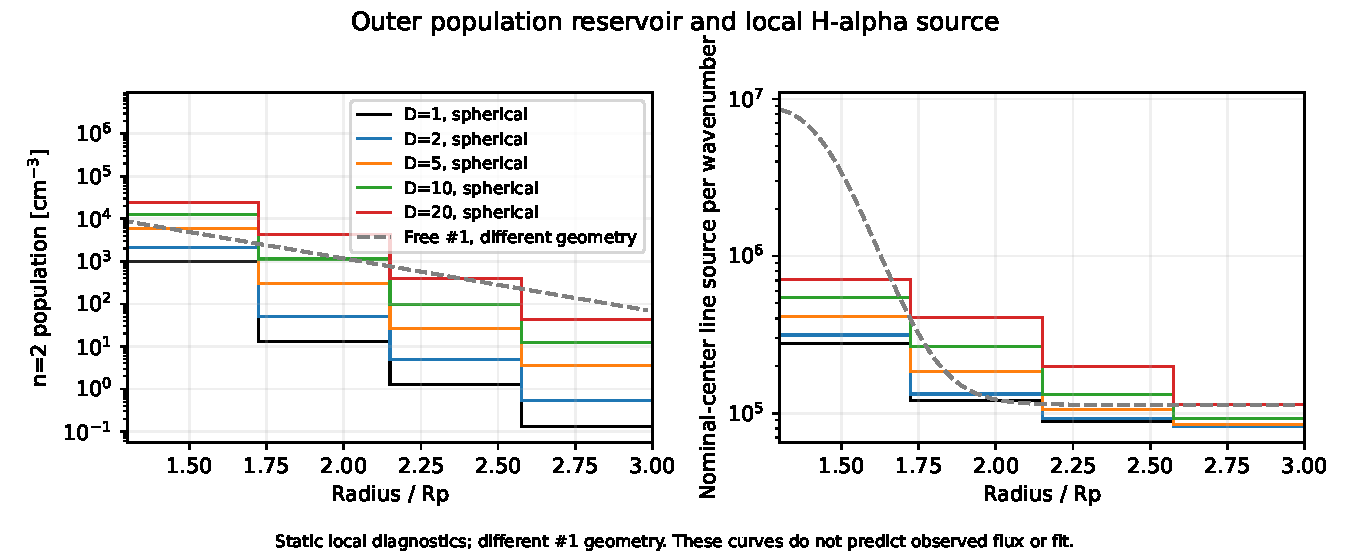
\includegraphics[width=0.98\linewidth]{../mceg/evidence/halpha_dense_outer_20261127/review/radial_structure.pdf}
\end{center}
The density family builds an absorbing reservoir, while the coupled source
brightens. The free model's sharp source transition and its different
geometry remain distinct. These static local curves do not predict the
observed residual; the native observer is evaluated separately.

\textbf{Why the fixed-bath expectation changes.}
At $D=5$, cell 5 has $22.83$ times the $n=2$ population of the matched
spherical $D=1$ root, but its H$\alpha$ source is also $1.54$ times larger.
The $n_3/n_2$ ratio becomes $1.51$ times its $D=1$ value. The stored upward $n=2\to3$
collisional rate is $4.13\times10^{-4}$ of the self-eliminated effective
radiative upward rate. This ratio alone does not establish the role of
collisions in the net balance, because large upward and downward rates can
cancel. The response is not simply heating: the cell's temperature decreases
from $D=3$ onward while its source increases.
The actual $n_3/n_2=0.00992$ is far below the same-temperature LTE value
$0.1582$ computed from the native atomic levels, so the state remains
strongly non-LTE.

The full profile-averaged H$\alpha$ intensity becomes about $1.57$ times
its $D=1$ value at $D=5$, but the dominant $3d$ branch's self-eliminated
effective upward and downward rates become $0.986$ and $0.638$ times their
$D=1$ values. Its own-branch source-elimination factor,
$(R_{\rm down}-R_{\rm stim})/A$, decreases from $0.967$ to $0.616$;
this is not a global escape probability or permanent photon-loss fraction.
The larger full intensity
must therefore not be described as a measured increase in effective external
pumping. These are correlated changes in a complete root, not a controlled
isolation of one causal channel. The earlier five-level bath also used the
pre-coupling PR13 reference; it is not the same reference radiation closure
as this $D=1$ control.
At $D=20$, the temperature at the same radius is slightly lower than at
$D=1$ ($7807$ versus $7898$ K), while $n_3/n_2$ is $3.30$ times larger.
The dominant $3d$ effective upward/downward coefficients become
$0.876/0.257$ times their $D=1$ values. The highest-density result therefore
also requires the coupled radiation/population response to be considered,
rather than attributing its brighter source to a higher temperature.
The $D=20$ ratio $n_3/n_2=0.02168$ remains below its same-temperature
LTE value $0.13582$, despite moving closer to LTE than the $D=1$ state.

\textbf{What the free model reveals.}
The free model's radial $n=2$ column above $1.725R_p$ is
$1.190\times10^{13}$ cm$^{-2}$. Matching that one integral does not match
the distribution at larger radius, the thermal line opacity, angular
emitting area or source function. More strikingly, the nominal-center source
ratio between $r=1.5125R_p$ and $1.9375R_p$ is $23.0$ in the free shape, compared with $2.31$
in the coupled $D=1$ root and $2.03$ at $D=10$. The dense family does not
automatically build that strong inner-to-outer brightness contrast.
The free shape has different geometry and additional freedoms, so this
comparison does not establish that the data uniquely require a ratio of 23.
Its source-departure transition is centered at $1.45R_p$ with scale
$0.08R_p$, inside the current broad cell spanning $1.3$--$1.725R_p$.
The present grid has not been shown to resolve such stratification. The
comparison therefore does not distinguish missing physics from structure
that the same physics might produce on a better resolved radial grid.

One additional observer case, $D=12$, was selected before inspecting its
residuals: among the accepted, CPU-verified $D=12$ and 15 states, it has the
smaller absolute log-distance to the free model's column above $1.725R_p$.
That column is $0.859$ times the free value, but the column above $2.15R_p$
is only $0.272$ times the free value. At $r=1.9375R_p$ the local $n=2$
population is $1.15$ times the free value; at $2.7875R_p$ it is only $0.136$
times the free value. This is an exploratory physical-column comparison,
not an exact match, a residual-selected optimum or a fitted density estimate.
After the matched observation processing and shared nuisance refit, its
blue-minus-core residual is $1725.56/1397.17$ ppm on primary/complementary
pixels: $23.96/19.42$ ppm worse than $D=1$. Its full-data score nevertheless
improves by $1.44/5.61$. Approaching the integrated outer column is therefore
insufficient in this prescribed family.
While the $D=20$ continuation was slow, $D=15$ was additionally selected as
the upper column bracket ($1.331$ times the free column). This adaptive
exploratory selection was recorded before evaluating its observer residuals;
it was not part of the earlier single-case selection rule.
Its blue-minus-core residual is $1740.74/1411.94$ ppm, respectively
$39.14/34.19$ ppm worse than $D=1$. The primary score is also worse by
$0.624$. Thus neither tested side of this column bracket improves the
target contrast.

\textbf{Why a smaller score is not yet the desired contrast.}
At $D=10$, profiling the same two shared RV/amplitude parameters reduces
the full-data score relative to $D=1$ by $2.95$ on primary pixels and $7.09$
on complementary pixels. Nevertheless, the absolute blue-minus-core
residual increases by $10.31$ and $6.77$ ppm, respectively. Both scores
remain worse than PR13. On primary pixels the processed planet-plus-GP
prediction changes by $-36.38/-26.07/+76.11$ ppm in B/C/R: the fitted core
darkens, but the blue peak weakens too. At fixed original nuisance parameters
the same changes are $-144.42/+11.50/+685.19$ ppm. Refitting both shared
parameters absorbs much of the response and changes its apparent shape.
These are predictions after native sampling and reference projection, not
intrinsic planetary fluxes; no disk/halo decomposition was performed.
At $D=20$, primary/complementary blue-minus-core residuals worsen by
$40.07/37.15$ ppm relative to $D=1$. The primary full-data score worsens by
$0.662$, while the complementary score improves by $2.455$; neither is a
contrast improvement. Relative to PR13 the scores are worse by
$66.645/57.357$. All recorded two-parameter fits succeed and remain well
inside the original parameter bounds. The sampled density family therefore
does not repair the observed contrast, even when it extends the static
absorption radius to the free model's value.

\textbf{Finite sensitivity controls.}
Increasing each observer ray-grid dimension by $1.5$ at the two phase nodes
bracketing the target changes profiled target predictions by at most
$0.243$ ppm. The blue-minus-core residual changes by only
$+0.0095/+0.0685$ ppm on primary/complementary pixels, leaving the outcome
unchanged. The other five phase nodes are identical. Four additional RV
starts for each pixel selection and both original/refined templates give
the same best scores within $5.9\times10^{-11}$. These are finite local
refinement and optimizer controls, not global error bounds.

At the exact $D=20$ state, doubling the H$\alpha$ transfer angle and frequency
quadrature changes non-LTE effective upward/downward rates by at most
$9.89\times10^{-10}$ and $8.89\times10^{-8}$. Doubling the wing domain
changes these rates by up to $1.57\times10^{-4}$, but cancellation makes
the summed net H$\alpha$ contribution to $n=3$ change by up to $1.37\%$
in non-LTE cells. The exposed partial H/free-free/redistribution heat changes
by up to $3.98\times10^{-5}$ of the saved thermal scale. The larger domain
also expands the background correction; it is not a pure line-wing change.
These fixed-state checks do not constitute a newly solved full atmosphere.
The saved isolated Stark midpoint proxy is at most $0.00451$ of an outer
own-branch source-elimination factor. That comparison does not bound the
collective net-rate response or validate a pressure-broadened line profile.

\textbf{Reproducibility and scope.}
The companion evidence directory retains exact accepted coordinates,
compact physical fields, CPU comparisons, native-observer receipts and
source hashes. The original large checkpoints and radiation dictionaries
are identified by path and hash. Interrupted continuation points remain
recorded as numerical failures to close, not as excluded physical models.
In particular, the first large step from $D=5$ to $D=10$ stalled; smaller
density steps reached a CPU-verified $D=10$ root with unchanged physics,
root-residual and physical acceptance criteria. A separate cancellation-aware
CPU comparison floor for the reference-force diagnostic is documented below;
it does not change the root criterion. The production source modules are unchanged.


\clearpage
\textbf{Precisely what is changed.}
For each trial temperature and composition, the existing transonic solver
produces reference profiles $\rho_0,v_0$ and the same pressure-to-density
profile $a^2=k_BT/(\mu m_p)$. Let
\[
 x=\operatorname{clip}\!\left(\frac{r/R_p-1.3}{0.425},0,1\right),\quad
 q=\exp\{\ln D\,x^2(3-2x)\},\qquad
 \rho=q\rho_0,\quad v=\frac{v_0}{q}.
\]
Thus $4\pi r^2\rho v=\dot M$ is unchanged, and
$\partial_r\ln v=\partial_r\ln v_0-\partial_r\ln q$.
The multiplier is relative to the reference wind \emph{at the new $T,\mu$},
not to the original saved density. Even inner cells with $q=1$ can respond
indirectly through that wind. The lower boundary and existing atomic/thermal
masks are retained. The density transition is sampled by one cell center on
the current eight-cell grid; resolving a physical transition is a separate task.

All native species and receiving channels participate in the new residual,
including the high hydrogen levels, metals, helium, molecules and the
charge-derived electron abundance. Spherical H$\alpha$ population transfer
is retained at every density. Other radiation, including continuum and
Ly$\alpha$, retains its native closure; this does not make all transport
spherical or three-dimensional. The $D=1$ solution is therefore compared both
to the new density cases and to the earlier PR13 atmosphere, which used a
different H$\alpha$ population-transfer closure.

\textbf{Thermal and force accounting.}
The same native flow-energy terms receive the modified velocity gradient.
At fixed $T,\mu$, $\rho v$ is unchanged, so thermal advection is unchanged;
the expansion term gains
\[
 \Delta Q_{\rm exp}=\rho_0v_0 a^2\partial_r\ln q.
\]
This term can be positive compression heating. It is not clipped or replaced
by a simple cooling multiplier. The additional acceleration required relative
to the reference momentum equation is
\[
 \Delta f=(v^2-v_0^2)\partial_r\ln v_0
              +(a^2-v^2)\partial_r\ln q.
\]
The reference solver's finite sampled momentum defect is retained separately
and added when reporting the total required acceleration. Reference wind
validity is not a momentum-validity claim for the modified flow. The force
can change sign with radius; a single magnetic-pressure estimate does not
establish its realization. Mechanical work $\rho v\Delta f$ is not silently
added as heat. A physical support mechanism must specify its energy exchange
and any dissipation. The native local-SE thermal closure also omits advected
excitation/ionization energy.

\textbf{What the numerical and observational checks establish.}
The complete 8,840-component residual must be below $10^{-9}$, a fresh
evaluation must repeat within $10^{-10}$, and all native transport/domain
guards must pass. Nuclear, charge, pressure and mass-flux consistency must
hold to $10^{-12}$. CPU checks evaluate exact saved coordinates without
polishing. The cancellation-dominated reference momentum defect uses an
absolute comparison floor of $10^{-12}$ times the uncancelled force scale;
the full residual, conservation and thermal criteria are unchanged.
Initial import/serialization failures and any unavailable density
stages are recorded separately from accepted roots.

The observer includes both the disk and off-limb emission. It retains native
samples, the stellar mask, common reference, fixed GP hyperparameters and
the same two global RV/amplitude nuisance parameters. Conditional GP means
are recomputed for changed templates. Target residuals use the same twelve
complete-band first-night exposures at $\phi=0.3761496$--$0.3932226$:
B=$[-40,-16)$, C=$[-8,8)$, R=$[16,40)$ km/s. Complete blue support is absent
on the second night. The score and selected-phase residuals are descriptive;
correlated pixels and uncalibrated extraction/time covariance still prevent
a significance or unique physical attribution.

Static CRD H$\alpha$ population transport uses natural/thermal broadening.
The observer uses the same width prescription.
Its adequacy at the new densities, nonlocal Ly$\alpha$ closure, radial
resolution, support stability and angular covering remain unqualified.
MCEG separates successful conditional numerical solves, measured native
comparisons and the physical realization of the supporting mechanism.
\end{document}
